In this chapter, we verify whether the developed multi-view clustering tool works as intended. It is important to show this to the reader in order to enhance the reliability of the results. To do this, we developed a sample application called PyPetstore. Since we are the experts of this application, we know what our multi-view clustering tool should output. Knowing this, we can verify the tool by comparing the expected outcome with the actual outcome. We also make small variations in PyPetstore, to see how the tool responds to it. This kind of test is called metamorphic testing in the domain of software engineering. In the next section, we first explain the structure and rationale behind PyPetstore. After this, we present the results when applying the multi-view clustering tool on different variations of PyPetstore.

\section{PyPetstore}
PyPetstore\footnote{\href{https://github.com/larsvasseldonk/PyPetstore}{https://github.com/larsvasseldonk/PyPetstore}} is a very simple command-line tool written in Python that helps managing the process of selling pets. The application is inspired by JPetstore\footnote{\href{https://github.com/mybatis/jpetstore-6}{https://github.com/mybatis/jpetstore-6}}, a Java application that is often used in related papers to validate the working of their approach \cite{al2021microservice, jin2018functionality, jin2019service, saidani2019towards, zhang2020automated}. 
In PyPetstore, users are able to create orders, add products to it, manage the availability of products, and get an overview of its customer base. The data acquired by the application is save into a SQLite database.
The application is implemented in seven modules, where each module implements the following functionality.

\begin{enumerate}
    \item \textbf{Customer.} The customer module allows users to create, update, delete, view, and search for customers in the database.
    \item \textbf{Database.} The database module initialises the database and its corresponding tables and is responsible for the database connection.
    \item \textbf{Order.} The order module enables users to create, view and search for orders in the database.
    \item \textbf{Orderdetail.} The orderdetail module assures that products can be added to an order. It is able to create and view order details.
    \item \textbf{Product.} The product module manages the product entities in the database. The module is able to create, delete, view and search for products.
    \item \textbf{Util.} This module contains some utility functions like the menu printing function.
    \item \textbf{Main.} The main module holds the application together. The main implements the workflow of the application.
\end{enumerate}

In total, PyPetstore consists of 8 modules, 5 classes, 18 functions and 40 methods and has 556 Lines of Code (LoC), comments excluded. 

\section{Metamorphic tests}
To test whether our multi-view clustering tool works, we apply the tool on different variations of PyPetstore. The resulting decompositions are then analysed and compared to the decomposition resulting from the original PyPetstore version. The following variation of PyPetstore are made.

\begin{itemize}
    \item \textbf{Swapping content.} In the first variation of PyPetstore, the original application is changed by swapping two top-level code fragments with each other. The code fragments are only swapped, and thus the content of the two code fragments stays the same. This means that also the static, semantic, and dynamic dependency should be identical. In addition, this also means that the resulting decomposition should be exactly the same as the one resulting from the orginal PyPetstore version.
    \item \textbf{Adding dependencies.} To verify if the tool resembles the correct top-level code fragments dependencies, we change the original PyPetstore version in a way the tool is forced discover new dependencies. These new dependencies that we manually instrumented in PyPetstore, should also be reflected in the new decomposition. 
\end{itemize}

In the next sections, we discuss the results of the tests regarding the static, semantic and dynamic dependencies.

\subsection{Verifying static dependencies}
Figure \ref{fig:pypestore_static_swapping_before} shows the graph constructed from the original PyPetstore version with only static dependencies. Each node in the graph represents a top-level code fragments, and the color shows to which service it belongs. The decomposition made with only static information results in four services. The decomposition seems appropriate to us, as it binds code fragments together that are related to each other. The module 'order', e.g., contains functionalities to create, view and delete orders and therefore makes several invocations to the 'Order' class. To create an order, it is also necessary to link a 'Customer' object to it. For this reason, we see in the static graph a dependency between the 'order' and 'Customer' code fragments. We also observe that this dependency is less strong, which makes sense since 'order' only invocates one time the 'Customer' class while it invocates three times the 'Order' class. For this reason, the edge weight between 'Order' and 'order' is much higher than the edge weight between 'order' and 'Customer'. Another important observation is that the graph gives high edge weights for edges within a service and low edges weights for edges between services. This is desirable as it increases the structural modularity quality (SMQ) of the decomposition.

\paragraph{Swapping content}
As mentioned before, we swap the 'Order' class with the 'Orderdetail' class and verify how our tools responds to it in terms of its static decomposition. Figure \ref{fig:pypestore_static_swapping_after} shows the new decomposition, and we can directly see it is slightly different than the decomposition of the original PyPetstore version. Instead of four candidate microservices, the application is now divided into three services. A potential reason for this could be the decreased dependency strength between the 'orderdetail' module and the 'Orderdetail' class, something that should not be possible. When looking into this, we notice that the 'orderdetail' module only makes two calls to the 'Orderdetail' class, while before there were four. We think the reason for this is that objects assigned to variables and then invoked are not considered by the call graph generator when the object is not defined in the same module. This way, the 'Orderdetail' class which is assigned to the variable 'orderdetail' and then called with 'orderdetail.printNicely' and 'orderdetail.toDb' are not discovered by the call graph generator, unless the 'Orderdetail' class is defined in the same module. This is a limitation of the call graph generator and is outside our control.\par

Despite this change, the other services of the new decomposition show a similar pattern as the original decomposition. The 'customer' module and 'Customer' class still have a high dependency, and the same is true for the 'product' and 'Product' code fragments. For this reason, even though the decomposition of the manipulated version is slightly different than before, we mark this test as completed. \par

\begin{figure}[h]
    \caption[The static graph of PyPetstore before and after swapping content.]{The static graph of PyPetstore (a) before and (b) after swapping the top-level code fragments 'Order' and 'Orderdetail'.}
    \label{fig:pypestore_static_swapping}
    \begin{adjustbox}{center}
    \begin{subfigure}{.5\textwidth}
        \caption{The original PyPetstore version}\label{fig:pypestore_static_swapping_before}
        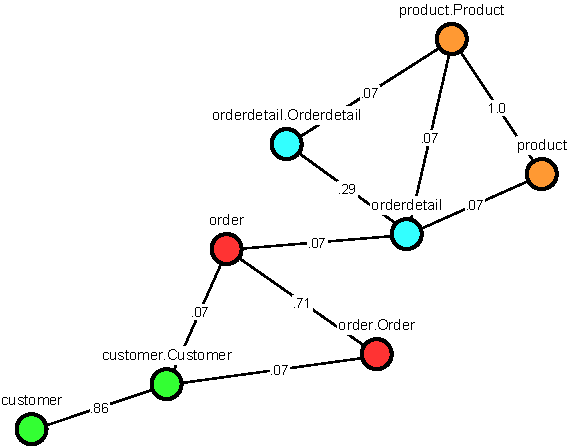
\includegraphics[width=200pt]{figures/data/pypetstore_static_original.pdf}
    \end{subfigure}
    \begin{subfigure}{.5\textwidth}
        \caption{The adjusted PyPetstore version}\label{fig:pypestore_static_swapping_after}
        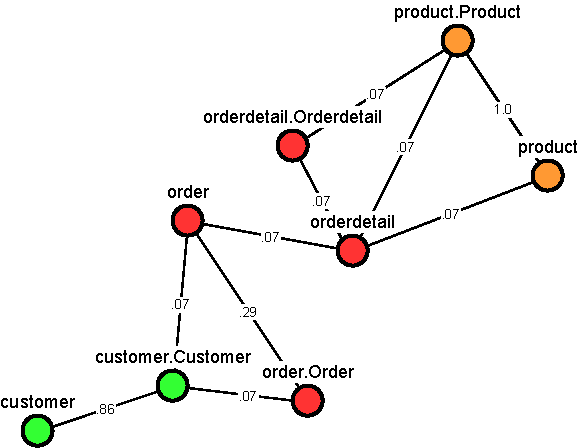
\includegraphics[width=200pt]{figures/data/pypetstore_static_swapped.pdf}
    \end{subfigure}
    \end{adjustbox}
\end{figure}

\begin{figure}[h]
    \caption[The static graph of PyPetstore when manually adding a static dependency.]{The static graph of PyPetstore when an extra call is added from 'order' to 'Product'. The left graph (a) only reflects one call between 'order' and 'Product' while the right graph (b) represents two calls.}
    \label{fig:pypetstore_static_extra_dependencies}
    \begin{adjustbox}{center}
    \begin{subfigure}{.5\textwidth}
        \caption{The adjusted PyPetstore version with one extra dependency.}\label{fig:pypetstore_static_extra_dependencies_1}
        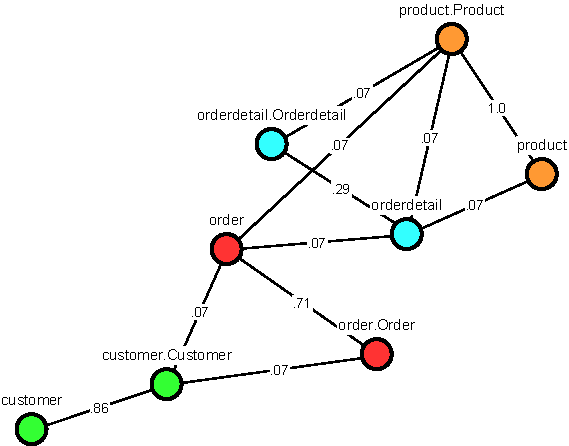
\includegraphics[width=200pt]{figures/data/pypetstore_static_1_added_depend.pdf}
    \end{subfigure}
    \begin{subfigure}{.5\textwidth}
        \caption{The adjusted PyPetstore version with two extra dependencies.}\label{fig:pypetstore_static_extra_dependencies_2}
        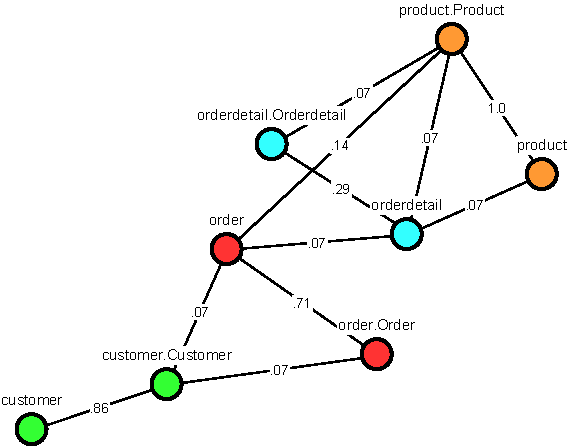
\includegraphics[width=200pt]{figures/data/pypetstore_static_2_added_depend.pdf}
    \end{subfigure}
    \end{adjustbox}
\end{figure}

\paragraph{Adding extra dependencies}
In the second verification test, we adjust the codebase by making a call from the 'order' module to the 'Product' class. The original PyPetstore version does not contain this dependency, and thus we should see a change in the resulting graph. The new decomposition is given in Figure \ref{fig:pypetstore_static_extra_dependencies_1}. When observing this new graph, we notice that indeed a new edge is added between the 'order' module and the 'Product' class. To see how the weight of the edge is determined, we made another variation of PyPetstore where a second call from the 'order' module to the 'Product' graph is added. The resulting graph, shown in Figure \ref{fig:pypetstore_static_extra_dependencies_2}, is similar as before, but the weight between 'order' and 'Product' is increased from a value of 0.7 to 0.14. This is as expected and verifies that the tool works as intended.

\subsection{Verifying semantic dependencies}
The decomposition that results from the original PyPetstore application is given in Figure \ref{fig:pypestore_semantic_before_after}. The figure shows that our tool generates four candidate microservices when only semantic dependencies are included. When comparing it to previous graphs, we see that the semantic graphs contains three additional code fragments, the 'database' module, 'Database' class and the 'main' module. This is possible since code fragments do not necessary need to be invocated by others. The semantic decomposition of the original PyPetstore version is reasonable since we see that semantic related code fragments, such as 'customer' and 'Customer' and 'product' and 'Product', are clustered together. 

\paragraph{Swapping content}
To verify the semantic analyser, we obtain again the decomposition of the adjusted PyPetstore version where the 'Order' and 'Orderdetail' code fragments are swapped. The resulting decomposition appears to be identical to the one in Figure \ref{fig:pypestore_semantic_before_after} and is for this reason not visualised again. This means that swapping code fragments does not influence the result and thus increases the reliability of the tool. \par

\begin{figure}
    \caption[The semantic graph of PyPetstore before and after swapping content.]{The semantic graph of the original and swapped version of PyPetstore. We only show one graph because both appear to be identical.}
    \label{fig:pypestore_semantic_before_after}
    \begin{adjustbox}{center}
    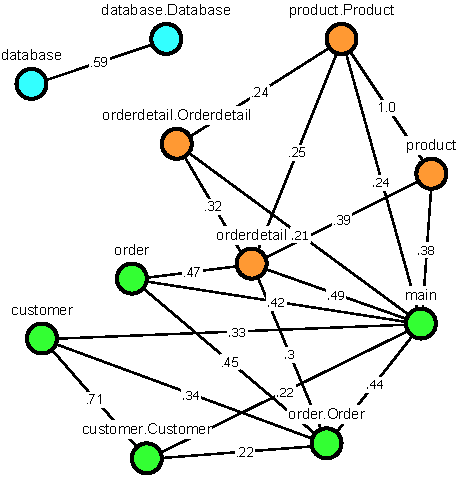
\includegraphics[width=200pt]{figures/data/pypetstore_semantic_original.pdf}
    \end{adjustbox}
\end{figure}

\paragraph{Adding extra terms}
The second test we run is to see how the tool deals with new domain terms. For this reason, we add five times the word 'database' to the 'database' and the 'main' module. With these new terms, we would expect that a new edge arises between the 'main' module and the 'database' module. When observing the new decomposition, we notice that adding the term 'database' does not result in a new semantic dependency. This is because the word database appears very frequently in the program since every module relies on the database. This high term frequency in the program results in a low tf-idf score and therefore does not exceed the threshold value of 0.05. \par
Now, let's try the same, but then with a more discriminate term like 'paper'. Figure \ref{fig:pypetstore_semantic_graph_after_add_terms} shows that indeed a new edge is created now, with a weight of 0.26. This is as expected and thus the test has succeeded.

\begin{figure}
    \caption{The semantic graph of PyPetstore after adding the term 'paper' five times in 'main' and 'database'.}
    \label{fig:pypetstore_semantic_graph_after_add_terms}
    \begin{adjustbox}{center}
    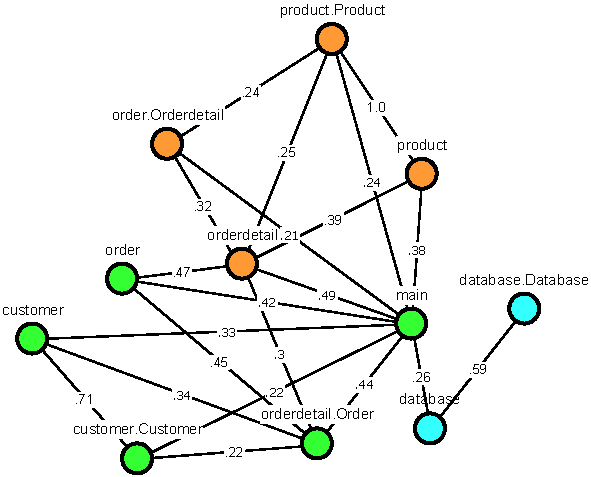
\includegraphics[width=300pt]{figures/data/pypetstore_semantic_add_depend.pdf}
    \end{adjustbox}
\end{figure}

\subsection{Verifying dynamic dependencies}
The decomposition of the original PyPetstore version constructed with dynamic dependencies is given in Figure \ref{fig:pypestore_dynamic_before}. The dynamic decomposition results in four services and is the only decomposition that also included the 'util' module. 

\paragraph{Swapping content}
Also for the dynamic dependency graph, we verify how it copes with code fragments that are swapped. Important for this test is that both the manipulated and the original PyPetstore versions are ran on the same test scenarios. This way, they both have the same logs and thus should make the same decomposition. The results, given in Figure \ref{fig:pypestore_dynamic_before}, show that both decompositions are identical. Since both decompositions are identical, we only visualised one in Figure \ref{fig:pypestore_dynamic_before}.

\paragraph{Adding extra test scenarios}
For the last verification test, we give the adjusted PyPetstore version two times the log files. This means that the expected outcome would be the exact same decomposition. This is because the strength of the edges are normalised, and thus a higher frequency cannot be seen from the graph. The result decomposition when adding twice the log files are identical to the one given in Figure \ref{fig:pypestore_dynamic_before}.

\begin{figure}
    \caption[The dynamic graph of PyPetstore.]{The dynamic graph of the original and swapped version of PyPetstore. We only show one graph because both appear to be identical.}
    \label{fig:pypestore_dynamic_before}
    \begin{adjustbox}{center}
    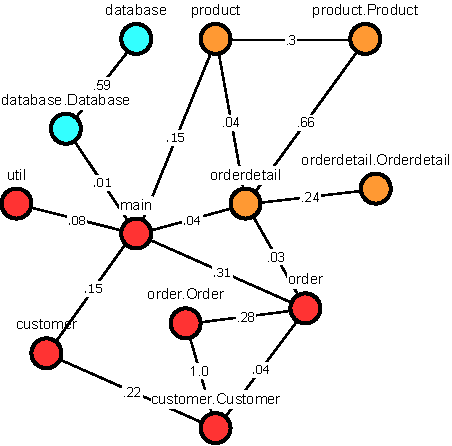
\includegraphics[width=200pt]{figures/data/pypetstore_dynamic_original.pdf}
    \end{adjustbox}
\end{figure}
